% !TeX root = main.tex
% !TeX spellcheck = fr_FR
\documentclass[12pt,a4paper,twoside]{article}
\usepackage[scaled]{helvet}
% Packages and macros
\usepackage[T1]{fontenc}
\usepackage{mathptmx}
\usepackage{pgf}
\usepackage{pgfpages}
\usepackage{parallel}
\usepackage{siunitx}
\usepackage{booktabs}
\usepackage{fancyhdr}
\usepackage{datetime}
\usepackage{multicol}
\usepackage{enumerate}
\usepackage{pifont}
\usepackage{amssymb}
\usepackage[export]{adjustbox}
\usepackage[margin=1in]{geometry}
\usepackage[french]{babel}
\usepackage{caption}
\usepackage{tikz}
\usepackage{tabularx}
\usepackage{gensymb}
\usepackage{hyperref}
\usepackage{graphicx}
\usepackage{pdfpages}
\usepackage{caption}
\usepackage{subcaption}
\usepackage{listings}
\usepackage{afterpage}

\usepackage{textcomp}

\newcommand{\source}[1]{\vspace{-11pt} \caption*{\small \textit{Source: {#1}} }}

\newcommand\blankpage{%
	\null
	\thispagestyle{empty}%
	\addtocounter{page}{-1}%
	\newpage}

\usepackage{verbatim}

\newdateformat{monthyeardate}{%
  \monthname[\THEMONTH], \THEYEAR}

\begin{document}
\pagestyle{fancy}
\lhead{PROJET 2221}
\chead {\today}
\rhead{LocalisationSousMarine}

% ------------------------- TITLE PAGE INSERTION ------------------------
\begin{titlepage} % Suppresses displaying the page number on the title page and the subsequent page counts as page 1
	\newcommand{\HRule}{\rule{\linewidth}{0.5mm}} % Defines a new command for horizontal lines, change thickness here
	
	\center % Centre everything on the page
	
	%------------------------------------------------
	%	Headings
	%------------------------------------------------
	
	\textsc{\LARGE Ecole des métiers de Lausanne \\ Ecole supérieure}\\[1.5cm] % Main heading such as the name of your university/college
	
	\textsc{\Large Génie électrique}\\[0.5cm] % Major heading such as course name
	
	\textsc{\large Système d'enregistrement de trajectoires de vol}\\[0.5cm] % Minor heading such as course title
	
	%------------------------------------------------
	%	Title
	%------------------------------------------------
	
	\HRule\\[0.4cm]
	
	{\huge\bfseries Boîte noire miniaturisée}\\[0.4cm] % Title of your document
	
	\HRule\\[1.5cm]
	
	%------------------------------------------------
	%	Author(s)
	%------------------------------------------------
	
	\begin{minipage}{0.4\textwidth}
		\begin{flushleft}
			\large
			\textit{Auteur}\\
			Ali \textsc{Zoubir} % Your name
		\end{flushleft}
	\end{minipage}
	~
	\begin{minipage}{0.4\textwidth}
		\begin{flushright}
			\large
			\textit{Superviseur}\\
			Juan José \textsc{Moreno} % Supervisor's name
		\end{flushright}
	\end{minipage}
	
	% If you don't want a supervisor, uncomment the two lines below and comment the code above
	%{\large\textit{Author}}\\
	%John \textsc{Smith} % Your name
	
	%------------------------------------------------
	%	Date
	%------------------------------------------------
	
	\vfill
	\vfill
	%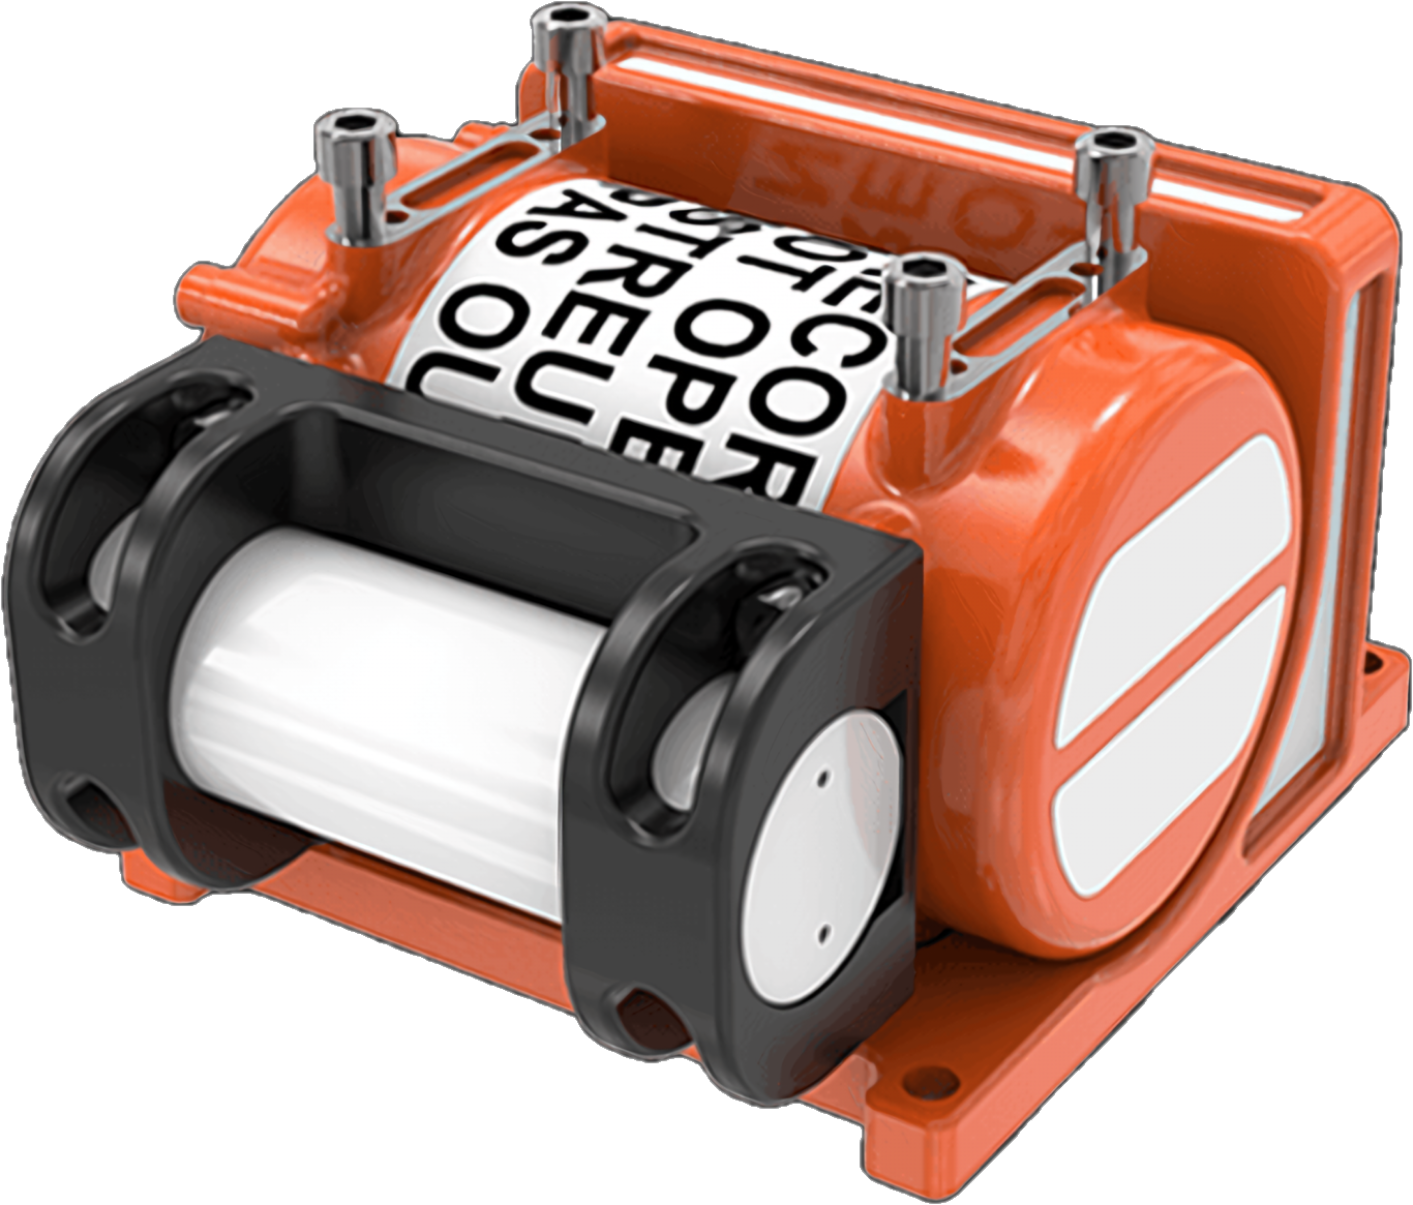
\includegraphics[width=5cm]{LOGO-PROJ}
	% \vfill\vfill\vfill % Position the date 3/4 down the remaining page
	\vfill
	
	{\large\today} % Date, change the \today to a set date if you want to be precise
	
	%------------------------------------------------
	%	Logo
	%------------------------------------------------
	
	%\vfill\vfill
	%\includegraphics[width=0.2\textwidth]{placeholder.jpg}\\[1cm] % Include a department/university logo - this will require the graphicx package
	
	%----------------------------------------------------------------------------------------
	
	\vfill % Push the date up 1/4 of the remaining page
	
\end{titlepage} 
\afterpage{\blankpage}

\clearpage

% --------------------- TABLE OF CONTENTS  ------------------------------- 
\tableofcontents
\clearpage


% ---- Bibliographie ----
%\input{bibliography}

\clearpage

\section{Conclusion}
{
	\paragraph{Synthèse} Le présent rapport a décrit le développement et la validation d'un projet de localisation sous-marine. L'objectif principal du projet était de concevoir et de mettre en oeuvre un système capable de collecter et de stocker des données de déplacement, de temps et de pression lors de plongées. Après avoir réalisé les différentes étapes de développement, nous pouvons conclure que le projet a été mené à une version finie.
	
	\paragraph{Développement} Au cours de la phase de développement, plusieurs étapes clés ont été franchies. Tout d'abord, une analyse approfondie des besoins et des contraintes a été réalisée, ce qui a permis de définir les spécifications du système. Ensuite, un processus itératif de conception a été suivi, comprenant la sélection des composants appropriés, la création des schémas électroniques, et la fabrication du prototype.
	
	\paragraph{Design} L'évaluation du design du projet a été effectuée en suivant une méthodologie rigoureuse de vérification et de validation. Les principales caractéristiques du projet, telles que les tensions d'alimentation, la communication UART et la communication SPI avec la carte SD, ont été vérifiées avec succès. Les mesures effectuées ont montré que le système fonctionnait correctement et répondait aux spécifications requises.
	
	\paragraph{Test} Le projet a été testé avec succès lors d'un enregistrement de données de déplacement pendant une durée de 5 heures, ce qui a permis de collecter 30 MB de données. Ces résultats confirment que le système est capable de fonctionner de manière fiable et de fournir les fonctionnalités attendues.
	
	\paragraph{Apports} Ce projet a permis d'acquérir une expérience précieuse dans le domaine de la conception et du développement de systèmes électroniques. Il a également mis en évidence l'importance de l'organisation, de la structure et de la vérification étape par étape des éléments du design.
	
	\paragraph{Correctifs} Afin de simplifier la mise en place du système, des correctifs mentionnés dans le fichier MODIF (Section \ref{ssec:Modif}) permettrait de palier a certaines erreurs non-critiques de développements.
	
	\paragraph{Améliorations} Des améliorations et des développements futurs peuvent être envisagés, tels que l'ajout de fonctionnalités supplémentaires, l'optimisation de la communication, l'extension des capacités de stockage ainsi que la mise en place d'une communication USB directement par le FTDI en corrigeant le pinning de SCK. Ces évolutions permettraient d'explorer de nouvelles possibilités d'application de ce système de localisation sous-marine.
	
	\paragraph{Remerciements} Je tiens à remercier sincèrement M. Juan José Moreno, mon responsable de projet, Dr. Gaston Baudat pour avoir mandaté le projet et pour sa contribution algorithmique sur la localisation, et M. Fréderic Mueller pour son aide mécanique et pour la conception de la rallonge du module. Leur soutien et leur expertise ont été essentiels pour mener à bien ce projet. Je suis reconnaissant de leur précieuse collaboration et de leurs conseils tout au long du processus.
	
	
}


\newpage
\nocite{*}
\section{Bibliographie}
\bibliography{Biblio-Proj} 
\bibliographystyle{ieeetr}

% ANNEXES
\clearpage
\section{Annexes}

\end{document}
